%*****************************************
\chapter{UML exercise one}\label{ch:uml}
%*****************************************

From the textual description of the use case the following use case diagram was derived:

\begin{figure}[H]
\begin{center}
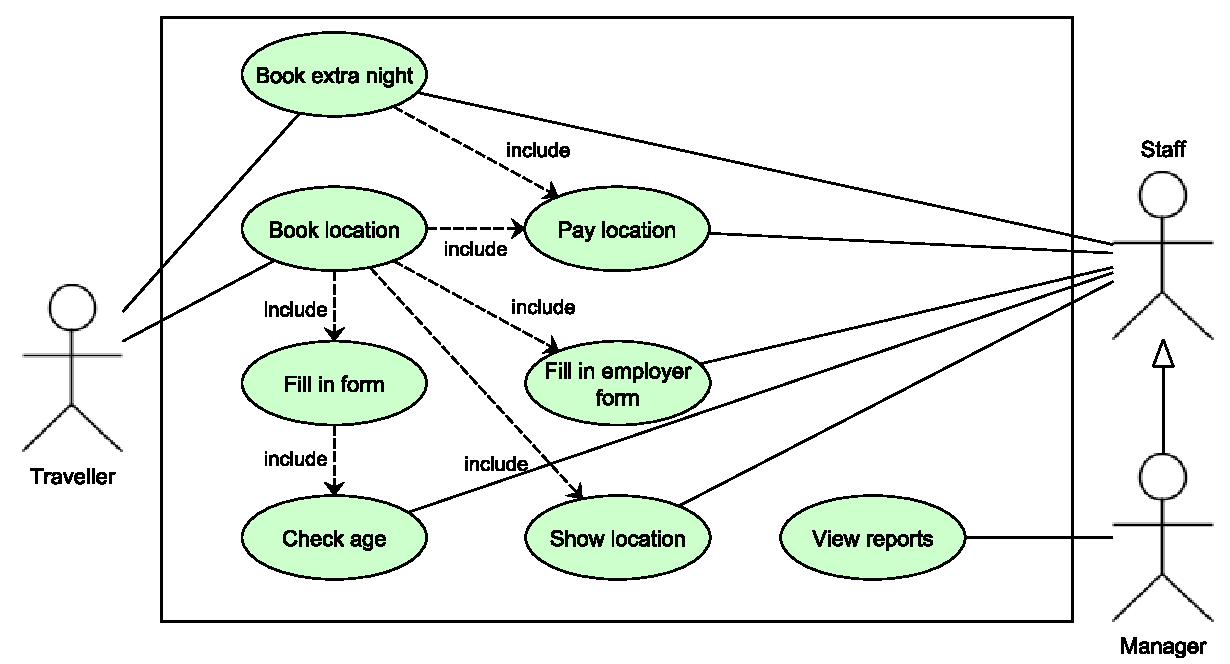
\includegraphics[width=\textwidth]{gfx/usecase.pdf} 
\end{center}
\caption{Use case diagram.}
\label{fig:usecase}
\end{figure}

The complexity level with many \textit{include} cases was choose to justify the use of a diagram and to show the possible sub-cases that might be reused.

Following from this description the \textit{book location} high-ceremony use case would look like the following scenario:

\section{High ceremony use cases}

\subsection{Use case: book location}

\begin{description}
\item[Goal:] Book a location.
\item[Actors:] Traveller, Staff.
\item[Precondition:] A location is available.
\item[Postcondition:] The traveller has booked a location for one night.
\item[Steps:]
\begin{enumerate}
\item Traveller \textit{fills in form}.
\item Staff \textit{fills in employer form}.
\item Traveller \textit{pays location}.
\item Staff \textit{shows location} to traveller.
\end{enumerate}

\item[Alternatives:]
\begin{enumerate}
\item[1A.] Fill in form use case fails.\\
The booking fails.
\item[3A.] Pay location use case fails.\\
The booking fails.
\end{enumerate}
\end{description}

\subsection{Use case: fill in form}

\begin{description}
\item[Goal:] Fill in form.
\item[Actors:] Traveller, Staff.
\item[Precondition:] User wants to book a location.
\item[Postcondition:] Form was filled in correct.
\item[Steps:]
\begin{enumerate}
\item Traveller enters personal details.
\item Traveller provides staff with passport.
\item Staff \textit{checks age}.
\item Staff returns passport.
\end{enumerate}

\item[Alternatives:]
\begin{enumerate}
\item[3A.] Check age use case fails.\\
The booking fails.
\end{enumerate}
\end{description}

\subsection{Use case: pay location}

\begin{description}
\item[Goal:] Pay for stay.
\item[Actors:] Traveller, Staff.
\item[Precondition:] -
\item[Postcondition:] -
\item[Steps:] -
\begin{enumerate}
\item Traveller pays for one night.
\item Staff accepts payment.
\item Staff marks payment as received.
\end{enumerate}

\item[Alternatives:]
\begin{enumerate}
\item[1A.] Traveller can not pay for stay.\\
The payment fails.
\end{enumerate}
\end{description}

\subsection{Use case: show location}

\begin{description}
\item[Goal:] Traveller is shown location.
\item[Actors:] Traveller, Staff.
\item[Precondition:] -
\item[Postcondition:] -
\item[Steps:] 
\begin{enumerate}
\item Staff shows traveller the location.
\end{enumerate}

\item[Alternatives:] -
\end{description}

\subsection{Use case: fill in employee form}

\begin{description}
\item[Goal:] Employee fills in form.
\item[Actors:] Staff.
\item[Precondition:] -
\item[Postcondition:] -
\item[Steps:] 
\begin{enumerate}
\item Staff enter details (location id, form number, nights to stay).
\end{enumerate}

\item[Alternatives:] -
\end{description}

\section{Activity diagrams}

\subsection{Book location}

\begin{figure}[H]
\begin{centering}
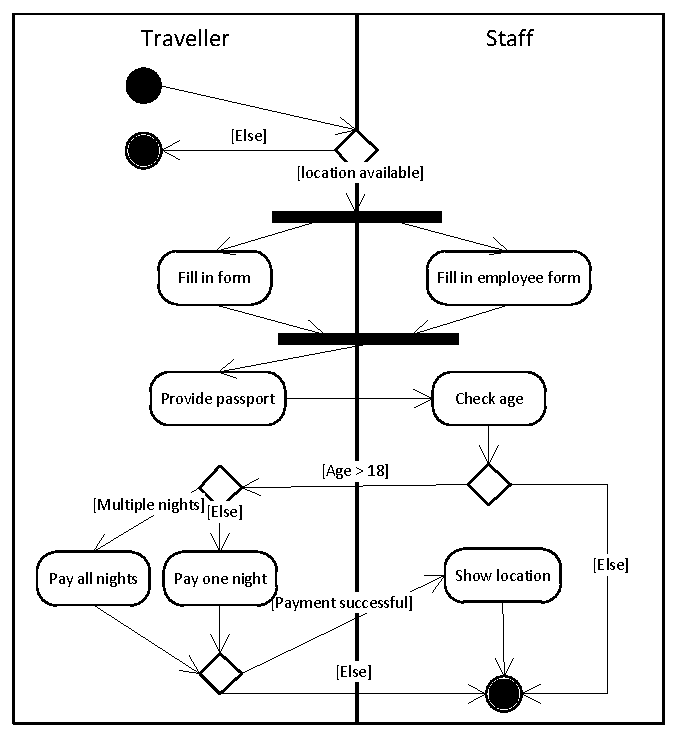
\includegraphics[width=\textwidth]{gfx/activity_diagram_book.pdf} 
\end{centering}
\caption{Activity diagram of book location.}
\label{fig:actdiag_book}
\end{figure}

Even though best practice is to only have one end-point per activity diagram, the provided activity diagram has two to improve readability.

\subsection{GetCost()}

\begin{figure}[H]
\begin{center}
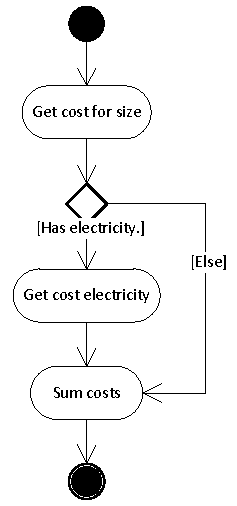
\includegraphics[scale=1]{gfx/activity_diagram_cost.pdf} 
\end{center}
\caption{Activity diagram of getCost for plots.}
\label{fig:actdiag_cost}
\end{figure}